\documentclass[12pt]{article}
\usepackage[a4paper, margin=1in]{geometry}
\usepackage{amsmath, amssymb, amsthm, tikz}



\begin{document}

\section*{Domácí série I}

Vypracoval: Daniel Ransdorf \hfill Podpis: \rule{4cm}{0.4pt}

\begin{enumerate}
  \item
    \begin{enumerate} 
      \item \textbf{Dilemma:}
        
        Pro $a,b,c,d,e,f \in \mathbb{N}$
        \[
        \frac{a+b+c+d+e+f}{\frac{1}{a}+\frac{1}{b}+\frac{1}{c}+\frac{1}{d}+\frac{1}{e}+\frac{1}{f}} = 2025
        \]

        \bigskip
      \item \textbf{Řešení:}
        \[
        a+b+c+d+e+f = \frac{2025}{a}+\frac{2025}{b}+\frac{2025}{c}+\frac{2025}{d}+\frac{2025}{e}+\frac{2025}{f}
        \]
        \[
        a - \frac{2025}{b} + b - \frac{2025}{a} + c - \frac{2025}{d} + d - \frac{2025}{c} + e - \frac{2025}{f} + f - \frac{2025}{e} = 0
        \]
        Chceme:
        \[
        a-\frac{2025}{b} = 0 \land b - \frac{2025}{a} = 0 \land c - \frac{2025}{d} = 0 \land \, ... \, \land f - \frac{2025}{e} = 0
        \]
        \[
        ab=2025 \land cd=2025 \land ef=2025
        \]
        Hledáme 3 páry přirozených čísel, jejichž součin je 2025.
        Vypišme dělitele čísla 2025 a zvolme 3 dvojice.

        \begin{align*}
          &1 \quad &3 \quad &5 \quad &9 \quad &15 \quad &25 \quad &27 \quad &45 \\
          &2025 \quad &675 \quad &405 \quad &225 \quad &135 \quad &81 \quad &75 \quad &45
        \end{align*}

        Zvolme například $(9,225) \, , \,  (15,135) \, , \, (25,81)$.
        \[
          \underline{\underline{a=9, b=225, c=15, d=135, e=25, f=81}}
        \]
        Tyto hodnoty splňují zadanou rovnost, zkouška:
        \begin{align*}
          \frac{9+225+15+135+25+81}{\frac{1}{9}+\frac{1}{225}+\frac{1}{15}+\frac{1}{135}+\frac{1}{25}+\frac{1}{81}} = 2025 \\
          \frac{490}{\frac{98}{405}}=2025 \\
          2025=2025       
        \end{align*}

    \end{enumerate}




















  \item
    \begin{enumerate} 
      \item \textbf{Tvrzení:}
        \[
        \forall f : \mathbb{R} \to \mathbb{R},\; f \text{ není konstantní} \;
        \exists x, y \in \mathbb{R} : f(x + y) < f(xy).
        \]
        
        \bigskip
      \item \textbf{Důkaz:}

        Předpokládejme opak, že existuje taková funkce, kde vztah neplatí
        \[
        \exists f_1 : \mathbb{R} \to \mathbb{R},\; f_1 \text{ není konstantní} \;
        \forall x, y \in \mathbb{R} : f_1(x + y) \geq f_1(xy)
        \]
        a dokažme, že $f_1$ musí být konstantní. Tím sporem dokážeme původní tvrzení.

        \medskip
        \textbf{1. krok} Ukázat, že $f_1$ je konstantní na intervalu $(-\infty, 0)$, neboli $\forall a<0:f_1(a) = f_1(0)$.

        \begin{itemize}
          \item Zvolme a dosaďme $x<0,y=0$: 
          \[f_1(x) \geq f_1(0) \quad \Rightarrow \quad f_1(a) \geq f_1(0), \; a<0
          \]

          \item Zvolme a dosaďme $y=-x$: 
          \[f_1(0) \geq f_1(-x^2) \quad \Rightarrow \quad f_1(0) \geq f_1(a), \; a<0
          \]

          \item Z předešlých dvou bodů plyne:
          \begin{align*}
            ( f_1(a) \geq f_1(0) ) \land ( f_1(0) \geq f_1(a) )&, \; a<0 \\
            \therefore f_1(a) = f_1(0)&, \; a<0
          \end{align*}
        \end{itemize}

        \medskip
        \textbf{2. krok} Ukázat, že $f_1$ je konstantní na intervalu $[0, +\infty)$, neboli $\forall a\geq0:f_1(a) = f_1(0)$.

        \begin{itemize}
          \item Zvolme a dosaďme $x\geq0,y=0$: 
          \[f_1(x) \geq f_1(0) \quad \Rightarrow \quad f_1(a) \geq f_1(0), \; a\geq0
          \]

          \item Zvolme a dosaďme $x\leq0,y<0$: 
          \begin{align*}
            &f_1(x+y) \geq f_1(xy) \\
            &\text{($x+y<0$, z 1. kroku plyne $f_1(x+y) = f_1(0)$)} \\
            &\Rightarrow f_1(0) \geq f_1(xy)\\
            xy\geq0 &\Rightarrow f_1(0) \geq f_1(a), \; a\geq0
          \end{align*}

          \item Z předešlých dvou bodů plyne:
          \begin{align*}
            ( f_1(a) \geq f_1(0) ) \land ( f_1(0) \geq f_1(a) )&, \; a\geq0 \\
            \therefore f_1(a) = f_1(0)&, \; a\geq0
          \end{align*}
        \end{itemize}

        \medskip
        \textbf{Finální úvaha:}
          Z předešlých dvou kroků víme:

          \begin{align*}
            &(\forall a<0: f_1(a) = f_1(0)) \land (\forall a\geq0: f_1(a) = f_1(0)) \\
            \Rightarrow \quad &\forall a \in \mathbb{R}: f_1(a) = f_1(0) \\
            \Rightarrow \quad &\forall a,b \in \mathbb{R}: f_1(a) = f_1(b) \\
            \Rightarrow \quad &\text{$f_1$ je konstantní na celém definičním oboru}
          \end{align*}

          V podmínkách opačného tvrzení je uvedeno, že $f_1$ není konstantní.
          Důkaz, že $f_1$ je konstantní, je spor opačného tvrzení.
          Tím je dokázana pravdivost původního tvrzení.
    
    \end{enumerate}
  









\item
    \begin{enumerate} 
      \item \textbf{Náčrt:}
      Označme délku hran čtvreců $a,b$.
      Za $a$ vždy zvolíme délku hrany většího čtverce, pokud čtverce nejsou stejné ($a \geq b$).
      Čtverce položíme do obdelníku tak, aby čtverec o hraně $a$
      na výšku "obklopoval" čtverec o hraně $b$,
      abychom zbytečně neprotahovali hrany obdelníku a tím zvyšovali obsah.
      
      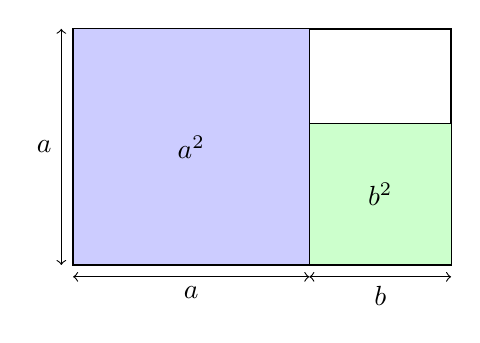
\begin{tikzpicture}[scale=3]
        % Parametry
        \def\a{1.0}       % strana většího čtverce
        \def\b{0.6}       % strana menšího čtverce

        % Obdélník o stranách (a+b) × a
        \draw[thick] (0,0) rectangle ({\a+\b},\a);
        % Velký čtverec vlevo
        \draw[fill=blue!20] (0,0) rectangle (\a,\a);
        \node at ({0.5*\a},{0.5*\a}) {$a^2$};
        % Menší čtverec vpravo
        \draw[fill=green!20] (\a,0) rectangle ({\a+\b},\b);
        \node at ({\a+0.5*\b},{0.5*\b}) {$b^2$};
        % Popisky rozměrů
        \draw[<->] (0,-0.05) -- (\a,-0.05) node[midway,below] {$a$};
        \draw[<->] (\a,-0.05) -- ({\a+\b},-0.05) node[midway,below] {$b$};
        \draw[<->] (-0.05,0) -- (-0.05,\a) node[midway,left] {$a$};
      \end{tikzpicture}

      \item \textbf{Pozorování:} 
      Jelikož $a \geq b$, obsah obdelníku bude mít vždy obsah $a(a+b)$.
      Chceme najít nejmenší obsah, se kterým sestrojíme obdelník, do kterého se vejdou oba čtverce.
      Jelikož maximum je nejmenší horní závorou, stačí nám najít maximální možný obsah obdelníku $a(a+b)$.
      Do čehokoli s menším obsahem se čtverce nevejdou, aniž by se překrývaly.
      Do čehokoli s větším obsahem se sice všechny možnosti vejdou, ale bude tam nadbytečné místo.
      Příklad převedeme na tyto výrazy. ($\uparrow$ znamená, že výraz chceme maximalizovat).

      \begin{align*}
        &\uparrow a(a+b) \quad , 0 < a,b < 1, a^2+b^2 = 1 \\
        &\uparrow a(a+b) \quad , 0 < a,b < 1, b = \sqrt{1-a^2} \\
        &\uparrow a(a + \sqrt{1-a^2}) \quad , 0 < a < 1 \\
        &\uparrow a^2 + a \sqrt{1-a^2}
      \end{align*}

      Nalezněme předpis změny hodnoty výrazu v závislosti na $a$:
      \begin{align*}
        \frac{d}{da} &= 2a + \frac{a}{2\sqrt{1-a^2}}(-2a) + \sqrt{1-a^2} \\
        \frac{d}{da} &= 2a + \frac{-a^2 + (1-a^2)}{\sqrt{1-a^2}} \\
        \frac{d}{da} &= 2a + \frac{1-2a^2}{\sqrt{1-a^2}} \\
      \end{align*}

      V maximu musí být $\frac{d}{da} = 0$.
      \begin{align*}
        2a_m + \frac{1-2a_m^2}{\sqrt{1-a_m^2}} &= 0 \\
        2a_m\sqrt{1-a_m^2} + (1-2a_m^2) &= 0 \\
        2a_m\sqrt{1-a_m^2} &= 2a_m^2-1 \quad (...^2)\\
        4a_m^2(1-a_m^2) &= (2a_m^2-1)^2 \\
        4a_m^2-4a_m^4 &= 4a_m^4 - 4a_m^2 + 1 \\
        0 &= 8a_m^4 - 8a_m^2 + 1 \quad (u:=a_m^2)\\
        0 &= 8u^2 - 8u + 1 \\
        a_m^2 = u_{1,2} &= \frac{8 \pm \sqrt{32}}{16} = \frac{1}{2} \pm \frac{\sqrt{2}}{4} \\
        &\text{($a$ je hrana většího čtverce, vybereme tedy větší hodnotu)} \\
        a_m^2 &= \frac{1}{2} + \frac{\sqrt{2}}{4} \quad \Rightarrow \quad a_m = \sqrt{\frac{1}{2} + \frac{\sqrt{2}}{4}} \\
        b_m &= \sqrt{1 - a_m^2} = \sqrt{1 - (\frac{1}{2} + \frac{\sqrt{2}}{4})} = \sqrt{\frac{1}{2} - \frac{\sqrt{2}}{4}}
      \end{align*}

      Dosazením bodů okolo zkontrolujeme, zda jsme skutečně našli maximum, ne minimum.

      \begin{align*}
        a_1^2 + a_1 \sqrt{1-a_1^2} \; &< \; a_m^2 + a_m \sqrt{1-a_m^2} \; > \; a_2^2 + a_2 \sqrt{1-a_2^2} \\
        a_1 &< a_m < a_2 \\
      \end{align*}
      \begin{align*}
        &\text{zvolme 0.1, 0.9} \\
        0.1^2 + 0.1 \sqrt{1-0.1^2} \; &< \; \frac{1}{2} + \frac{\sqrt{2}}{4} + \sqrt{\frac{1}{2} + \frac{\sqrt{2}}{4}} \sqrt{1-(\frac{1}{2} + \frac{\sqrt{2}}{4})} \; > \; 0.9^2 + 0.9 \sqrt{1-0.9^2} \\
        \frac{1+3\sqrt{11}}{100} &< \frac{1+\sqrt{2}}{2} > \frac{81+9\sqrt{19}}{100} \\
        0.109... &< 1.207... > 1.202...
      \end{align*}

      Skutečně jsme zvolili maximum, takže jsme našli nejvyšší možný obsah obalu těch dvou čtverců.
      Tím pádem řešením úlohy je:

      \[
      S = \frac{1+\sqrt{2}}{2}
      \]

      

    \end{enumerate}






  \setcounter{enumi}{4}

  \item
    \begin{enumerate} 
      \item \textbf{Tvrzení:}
        Pro libovolná přirozená čísla \(a,b,c\) existuje přirozené číslo \(n\),
        pro které výraz \(\sqrt{n^3 + a n^2 + b n + c}\) není celé číslo.
        
        \bigskip
      \item \textbf{Důkaz:}
        
        Uvažujme polynom
        \[
          P(n) = n^3 + a n^2 + b n + c.
          \]
          Chceme dokázat, že existuje \(n \in \mathbb{N}\), pro které \(P(n)\) není dokonalý čtverec.
          
          Protože každé celé číslo ve tvaru \(x^2\) dává po dělení 4 zbytek pouze \(0\) nebo \(1\),
          stačí ukázat, že existuje \(n\), pro které \(P(n) \equiv 2 \text{ nebo } 3 \pmod 4.\)
          
          \medskip
          Spočtěme zbytky polynomu \(P(n)\) modulo 4 pro několik po sobě jdoucích hodnot \(n\):
          
          \[
            \begin{aligned}
              P(1) &\equiv 1 + a + b + c \pmod 4,\\
              P(2) &\equiv 8 + 4a + 2b + c \equiv 2b + c \pmod 4,\\
              P(3) &\equiv 27 + 9a + 3b + c \equiv 3 + a - b + c \pmod 4,\\
              P(4) &\equiv 64 + 16a + 4b + c \equiv c \pmod 4.
            \end{aligned}
            \]
            
            \medskip
            Nyní rozlišíme případy podle zbytku čísla \(c\) po dělení 4.
            
            \begin{itemize}
              \item Pokud \(c \equiv 2\) nebo \(3 \pmod 4\), pak \(P(4) \equiv c \in \{2,3\}\),
              takže \(P(4)\) není kongruentní s žádným čtvercem modulo 4. 
              Tedy \(\sqrt{P(4)}\) není celé číslo.
              
              \item Pokud \(c \equiv 0\) nebo \(1 \pmod 4\), rozlišíme podle parity \(b\).
              \begin{itemize}
                \item Je-li \(b\) liché, pak \(P(2) \equiv 2b + c \equiv 2 + c \in \{2,3\}\),
                tedy \(P(2)\) není čtverec modulo 4.
                \item Je-li \(b\) sudé, potom \(P(2) \equiv c \in \{0,1\}\),
                takže se podívejme na \(P(1)\) a \(P(3)\):
                \[
                  P(1) \equiv 1 + a + c \pmod 4, \qquad
                  P(3) \equiv 3 + a + c \pmod 4.
                  \]
                  Tyto dva zbytky se liší o 2 modulo 4, tedy nemohou být oba v množině \(\{0,1\}\).
                  Z toho plyne, že alespoň jeden z nich je \(\equiv 2\) nebo \(3 \pmod 4\),
                  a tudíž odpovídající \(P(n)\) není čtverec modulo 4.
                \end{itemize}
              \end{itemize}
              
              \medskip
              Ve všech případech jsme nalezli alespoň jedno \(n \in \{1,2,3,4\}\),
              pro které \(P(n)\) není kongruentní s žádným čtvercem modulo 4.
              Proto \(\sqrt{P(n)}\) není celé číslo.
              
              \[
                \boxed{
                  \forall a,b,c \in \mathbb{N} \; \exists n \in \mathbb{N} :
                  \sqrt{n^3 + a n^2 + b n + c} \notin \mathbb{Z}.
                  }
                  \]
                  
                  \hfill\(\square\)
    \end{enumerate} 
  
\end{enumerate}

\end{document}
